
All regions defined in this analysis share a common lepton, jet, and overall event selection. This selection is detailed here; the selection used to define the various fit regions is described in section \ref{sec:signal_region}.

\subsection{Trigger}

Events are required to be selected by dilepton triggers, as summarized in table \ref{tbl:trigger}. \textbf{The 2018 trigger has not yet been implemented, and 2018 data currently uses 2017 triggers.}

\begin{table}[h!]
 \begin{center}
   \begin{tabular}{cc}
     \toprule
                  & Dilepton triggers (2015) \\
     \midrule
      $\mu\mu$ (asymm.)          & \verb!HLT_mu18_mu8noL1! \\
      $ee$ (symm.)               & \verb!HLT_2e12_lhloose_L12EM10VH! \\
      $e\mu,\mu e$ ($\sim$symm.) & \verb!HLT_e17_lhloose_mu14! \\
     \bottomrule
                       & Dilepton triggers (2016) \\
     \midrule
      $\mu\mu$ (asymm.)                   & \verb!HLT_mu22_mu8noL1! \\
      $ee$ (symm.)                        & \verb!HLT_2e17_lhvloose_nod0! \\
      $e\mu,\mu e$ ($\sim$symm.)          & \verb!HLT_e17_lhloose_nod0_mu14! \\
     \bottomrule

                  & Dilepton triggers (2017) \\
     \midrule
      $\mu\mu$ (asymm.)                   & \verb!HLT_mu22_mu8noL1! \\
      $ee$ (symm.)                        & \verb!HLT_2e24_lhvloose_nod0! \\
      $e\mu,\mu e$ ($\sim$symm.)          & \verb!HLT_e17_lhloose_nod0_mu14! \\
     \bottomrule
   \end{tabular}
   \caption{\label{tbl:trigger} List of lowest $p_{T}$-threshold, un-prescaled dilepton triggers used for 2015-2017 data taking.}
 \end{center}
\end{table}

\subsection{Light leptons}
\label{subsec:leps}

Electron candidates are reconstructed from energy clusters in the electromagnetic calorimeter that are associated with charged particle tracks reconstructed in the inner detector~\cite{ATLAS-CONF-2016-024}.  Electron candidates are required to have $\pt > 10$ GeV and $|\eta_\textrm{cluster}| < 2.47$. Candidates in the transition region between different electromagnetic calorimeter components, $1.37 < |\eta_\textrm{cluster}| < 1.52$, are rejected. A multivariate likelihood discriminant combining shower shape and track information is used to distinguish real electrons from hadronic showers (fake electrons). To further reduce the non-prompt electron contribution, the track is required to be consistent with originating from the primary vertex; requirements are imposed on the transverse impact parameter significance ($|d_0|/\sigma_{d_0}$) and the longitudinal impact parameter ($|\Delta z_0 \sin \theta_\ell|$), as shown in table \ref{tbl:tightleps}. 
                   
Muon candidates are reconstructed by combining inner detector tracks with track segments or full tracks in the muon spectrometer \cite{PERF-2014-05}. Muon candidates are required to have $\pt > 10$~GeV and $|\eta| < 2.5$. 

All leptons are required to be isolated, and pass a non-prompt BDT selection described in detail in \cite{ttH_paper}. 

\begin{table}
\begin{center}
 \begin{tabular}{l|cccccc}
 \hline\hline
 & \multicolumn{3}{c|}{$e$} & \multicolumn{3}{c}{$\mu$} \\
 \hline
 & L & L* & T & L & L* & T \\
  \hline
  FixedCutLoose           &  No & \multicolumn{2}{|c|}{Yes} & No & \multicolumn{2}{|c}{Yes} \\
  \hline
  Non-prompt lepton BDT   &  \multicolumn{2}{c|}{No} & \multicolumn{1}{c|}{Yes} & \multicolumn{2}{c|}{No} & \multicolumn{1}{c}{Yes} \\
  \hline
  Identification  & \multicolumn{2}{c|}{Loose} & \multicolumn{1}{c|}{Tight} & \multicolumn{2}{c}{Loose} & Medium\\
  \hline
  Charge mis-assignment veto &  \multicolumn{2}{c|}{No} & Yes & \multicolumn{3}{|c}{N/A} \\
  \hline
  ambiguity bit == 0 &  \multicolumn{2}{c|}{No} & Yes & \multicolumn{3}{|c}{N/A} \\
  \hline
  Transverse impact parameter significance  &  \multicolumn{3}{c|}{$<5$} & \multicolumn{3}{c}{$<3$ } \\
  $|d_0|/\sigma_{d_0}$ & \multicolumn{3}{c|}{} &  \multicolumn{3}{c}{}  \\
  \hline
  Longitudinal impact parameter &  \multicolumn{6}{c}{$< 0.5$ mm} \\
  $|z_0 \sin \theta|$ &  \multicolumn{6}{c}{} \\
  \hline\hline
 \end{tabular}
\caption{\label{tbl:tightleps} Loose (L), loose and minimally-isolated (L*), and tight (T) light lepton definitions.}
\end{center}
\end{table}


\subsection{Jets}
\label{subsec:jets}

Jets are reconstructed from calibrated topological clusters built from energy deposits in the calorimeters \cite{ATL-PHYS-PUB-2015-015}, using the anti-$k_t$ algorithm with a radius parameter $R=0.4$.  Jets with energy contributions likely arising from noise or detector effects are removed from consideration \cite{ATLAS-CONF-2015-029}, and only jets satisfying $\pt > 25$~GeV and $|\eta| < 2.5$ are used in this analysis.  For jets with $\pt < 60$~GeV and $|\eta| < 2.4$, a jet-track association algorithm is used to confirm that the jet originates from the selected primary vertex, in order to reject jets arising from pileup collisions \cite{PERF-2014-03}.

\subsection{B-tagged Jets}
\label{subsec:bjets}

In order to make a measurement of $WZ$ + heavy flavor it is necessary to distinguish these events from $WZ$ + light jets. For this purpose, the MV2c10 b-tagging algorithm is used to distinguish heavy flavor jets from lighter ones. The MV2c10 algorithm uses jet kinematics, particularly jet vertex information, as input for a BDT which assigns each jet a score designed to reflect how likely that jet is to have originated from a b-quark. 

\begin{figure}[H]
    \centering
    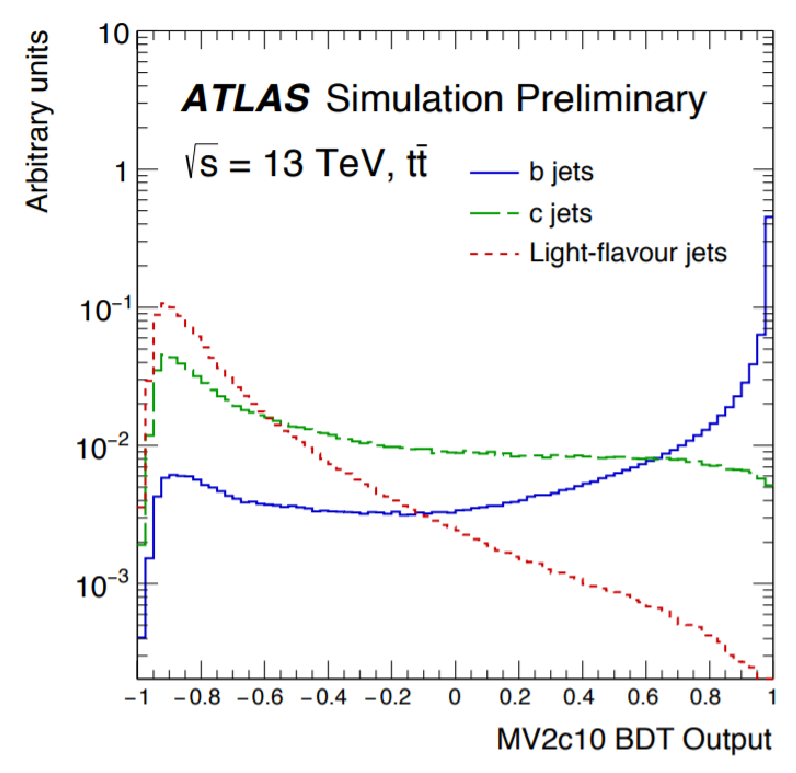
\includegraphics[width=0.54\linewidth]{MV2c10_output.eps}
    \caption{Output distribution of the MV2c10 algorithm for b-jets, charm jets, and light jets}
    \label{fig:MV2c10}
\end{figure}

From the output of the BDT, working points (WPs) are developed based on the efficiency of truth b-jets at particular values of the MV2c10 algorithm. The working points used in this analysis are summarized in table \ref{tab:btag_WPs}. 

\begin{table}[H]
\begin{center}
\begin{tabular}{|c|ccccc|}
    \hline
       WP &  none & loose & medium & tight & tightest\\
       \hline
     b eff. & - & 85\% & 77\% & 70\% & 60\% \\ 
    \hline
    \end{tabular}    
    \caption{B-tagging Working Points by tightness and b-jet efficiency}
    \label{tab:btag_WPs}
    \end{center}
\end{table}

A tighter WP will accept fewer b-jets, but reject a higher fraction of charm and light jets. Generally, analyses that include b-jets will use a fixed working point, for example, requiring that a jet pass the 70\% threshold. By instead treating these working point as bins, e.g. events with jets that fall between the 85\% and 77\% WPs fall into one bin, while events with jets passing the 60\% WP fall into another, and looking at the full psuedo-continuous MV2c10 spectrum of the jets, additional information can be gained. The psuedo-continuous b-tag spectrum is used in this case to separate out WZ + b, WZ + charm, and WZ + light. 

\subsection{Missing transverse energy}
\label{subsec:met}

Missing transverse momentum ($E_T^{miss}$) is used as part of the event selection. The missing transverse momentum vector is defined as the inverse of the sum of the transverse momenta of all reconstructed physics objects as well as remaining unclustered energy, the latter of which is estimated from low-\pt tracks associated with the primary vertex but not assigned to a hard object \cite{ATL-PHYS-PUB-2015-027}. 

